\documentclass[11pt,a4 paper,one side]{article}
\usepackage{amsmath,amssymb,graphicx}
\usepackage{ctex}  
\usepackage[colorlinks=true,linkcolor=red,citecolor=red,filecolor=magenta,urlcolor=cyan]{hyperref}
\usepackage{bookmark}
\usepackage{fontspec}
\setmainfont{Times New Roman}
\usepackage{xcolor}
\usepackage{geometry}
\geometry{a4paper, left=2.5cm, right=2.5cm, top=2.5cm, bottom=2.5cm}
\title{偏微分方程数值解+第二次上机作业}
\author{2100012131 蒋鹏}
\date{\today}
\begin{document}
\maketitle
\tableofcontents
\section{问题描述}
在指定区域上$\Omega$求解Robin边值问题的Laplace方程
\begin{align}
\begin{cases}
    -\Delta u=f, &x\in \Omega \\
    \alpha  u+\beta  \frac{\partial u}{\partial \vec{n}}=g, &x\in \partial \Omega
\end{cases}
\end{align}
其中区域$\Omega$如图\ref{Domain}所示。\begin{figure}
    \centering
    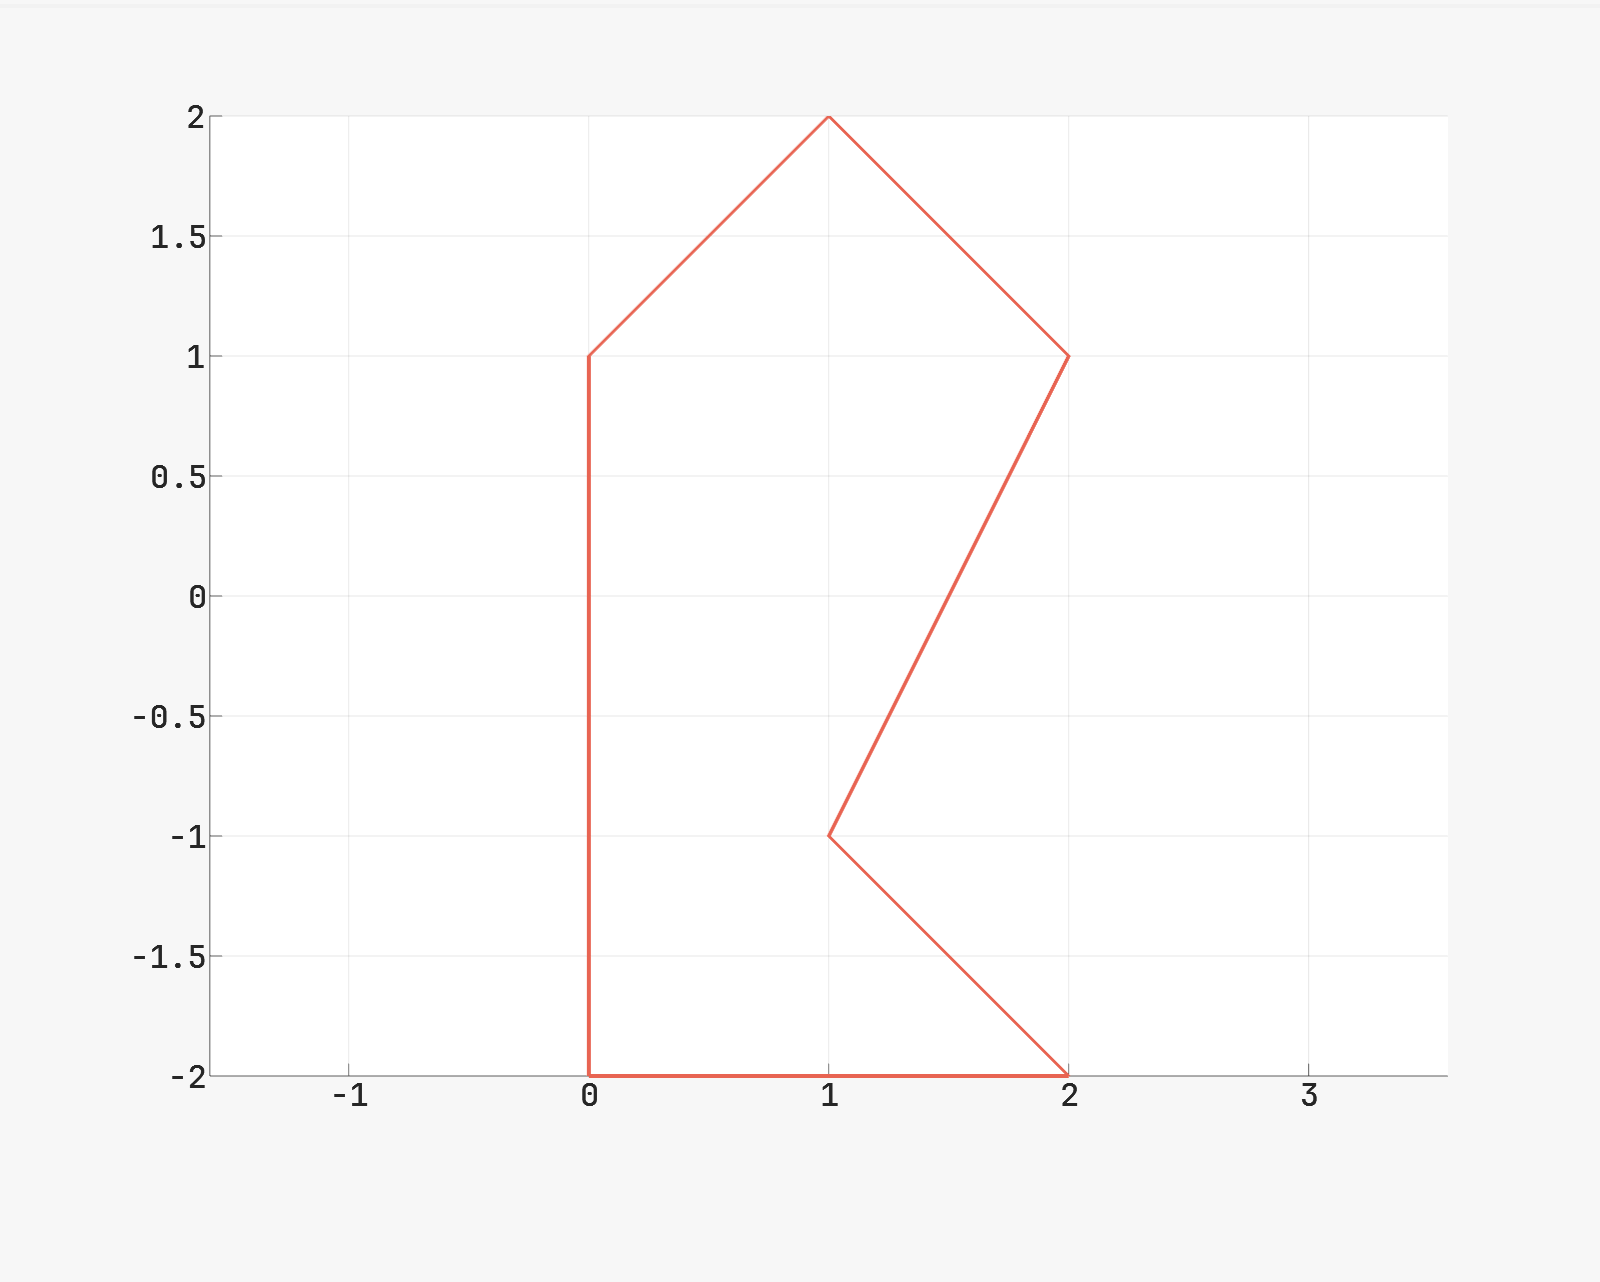
\includegraphics[width=0.9\linewidth]{Domain.png}
    \caption{Domain}
    \label{Domain}
\end{figure}
\section{算法设计}
\subsection{区域离散}
在$x$和$y$方向以相同尺度$h$进行均匀剖分。令$N=1/h$,自下而上,从左至右,对Domain内的点及边界点进行编号,$0\leq i \leq 4N$,$0\leq j \leq j\_num[i]$。
所有点可分为三类:内点,边界点及临边界点,角点。
\subsection{算子离散}
对于不同点进行不同格式离散:
\\ 对于内点,采取五点差分格式离散Laplace算子。
\\ 对于边界点,采取前向或者后向差商格式离散梯度,进而离散方向导数。
\\ 对于临边界点,即该点$(x,y)$非内点且不位于边界,则在边界上最近点为$(x^*,y^*)$,以点$(x,y)$的差商近似$(x^*,y^*)$的梯度,进而离散方向导数。
\\ 对于角点,我们规定其左侧边界为其外法向,于是所有角点有唯一外法向且每条边界有唯一端点与其同外法向。
\subsection{方程求解}
此线性方程组较为复杂,我们采取Gauss-Seidel的SOR迭代法进行求解。同时我们也采取了Jacobi迭代进行对比。此两种迭代法实现简单,只需在每次遍历中对每个点进行相应更新即可。
\\ 不采取共轭梯度法与多重网格算法的原因是:该方程组非对称正定,算法收敛性无保证。
\\ 可能的改进:Precondition,GMRES(m)
\section{数值实验}
\end{document}